\chapter{Experimental File System(eXpFS)}
\label{chap3}
\section{Introduction}
 
The eXpFS logical file system provides a file abstraction that allows application programs to think of each data (or executable) file stored in the disk as a continuous stream of data (or machine instructions) without having to worry about the details of disk block allocation. eXpOS provides a sequence of file system calls through which application programs can create/read/write files. These system calls are OS routines that does the translation of the user request into physical disk block operations.
\\
In addition to the eXpOS system call interface, the eXpFS specification also requires that there is an external interface through which executable and data files can be loaded into the file system externally. The external interface for eXpOS implementation on the XSM machine is the XFS Interface.
\\
This section discusses the abstract logical view provided by eXpFS to the eXpOS application programmer. 

\section{eXpFS File system organization}
The eXpFS logical file system comprises of files organized in a single directory called the root. The root is also treated conceptually as a file. Every eXpFS file is a sequence of words. Associated with each eXpFS file there are three attributes - name, size and type, each attribute being one word long. The filename must be a string. Each file must have a unique name. The size of the file will be the total number of words stored in the file.(The maximum size of a file is operating system dependent). There are three types of eXpFS files - the root, data files and executable files. Each file in eXpFS has an entry in the root called its root entry. 

\subsection{The eXpFS Root File}
The root file has the name root and contains meta-data about the files stored in the file system. For each file stored in eXpFS, the root stores three words of information - filename, file-size and file-type. This triple is called the root entry for the file. The first root entry is for the root itself. The order in which the remaining entries appear is not specified and can vary with the implementation. (The maximum size of the root file is defined by XFS\_ROOTSIZE.).
\\
Example: If the file system stores two files - a data file, file.dat, of size 700 words and an executable file, confirm this program.xexe, of 1025 words, the root file will contain the following information. 
\begin{figure}[ht]
\centering
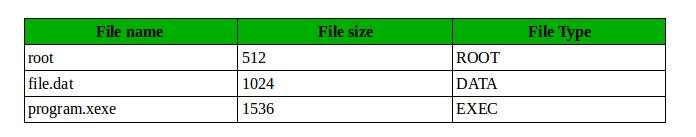
\includegraphics[scale=0.50]{figures/root_entry.jpg}
\caption{\footnotesize Root File Entry}
\label{fig_1}
\end{figure}

The operations on the root file are Open, Close, Read and Seek. 

\subsection{eXpFS Data files}
A data file is a sequence of words. The maximum number of words permissible in a file is defined by the constant MAX\_FILE\_SIZE. (It is a recommended programming convention to use the extension ".dat" for data files). eXpFS treats every file other than root and executable files as a data file. The Create system call automatically sets the file type field in the root entry for any file created through the create system call to DATA.
\\
eXpOS allows an application program to perform the following operations on data files: Create, Delete, Open, Close, FLock, FUnlock, Read, Write, Seek. Application programs can create only data files using the Create system call. In addition to this, data files may be loaded into the eXpFS file system using the external interface. 

\subsection{eXpFS Executable files}
 These contain executable code for programs that can be loaded and run by the operating system. From the point of view of the eXpFS file system alone, executable files are just like data files except that file type is EXEC in the root entry. eXpFS specification does not allow executable files to be created by application programs. They can only be created externally and loaded using the external interface. However, application programs can read or modify executable files like data files.
\\
Executable files are essentially program files that must be loaded and run by the operating system. Hence the Operating system imposes certain structure on these files (called the executable file format). Moreover, the instructions must execute on the machine on which the OS is running. Thus, there is dependency on the hardware as well. Typically, an application program written in a high level language (like ExpL ) is compiled using a compiler that generates the executable file. The compiler generates executable file that is dependent on the operating system as well as the target machine.
\\
An OS implementation on a particular machine specifies an application binary interface (ABI). The eXpOS ABI for XSM machine is described in Appendix A. Application programs are typically written in a high level language like ExpL. The ExpL compiler for eXpOS running on the XSM machine generates target code based on the ABI specification for eXpOS on XSM.
\\
The executable file format recognized by eXpOS is called the Experimental executable file (XEXE) format. In this format, an executable file is divided into two sections. The first section is called header and the second section called the code (or text) section. The code section contains the program instructions. The header section contains information like the size of the text and data segments in the file, the space to be allocated for stack and heap areas when the program is loaded for execution etc. This information is used by the OS loader to map the file into a virtual address space and create a process in memory for executing the program.
\\
An application program can read/modify an executable file like a data file using the standard system calls on data files. In addition to this, the Exec system call invokes the eXpOS loader that loads an executable file in XEXE format into memory for execution. 
